This section specifies the software architecture requirements and the software
architecture design at the second level of granularity - the benchmark service
of the benchmarking system. The benchmrk service will be responsible for monitor
program that will be run within a linux contatiner, which will monitor the users program.

\section{Overall Software Architecture}
\subsection{Architecture Requirements}
This section discusses the software architecture requirements around the
backend benchmark system infrastructure. The backend benchmark system will be
responsible for creating a linux container which will hold the monitor program
which will monitor the users program instance. In particular
the architecture requirements at the second level of granularity is specified.

The architecture requirements should specify:
\begin{itemize}
	\item the architectural responsibilities which need to be addressed
	\item the access and integration requirements for the system
	\item the quality requirements
\end{itemize}

Figure \ref{fig:benchmarkInfrastructure} show the a high-level infrastructure
view of the Benchmark service.

\begin{figure}[H]
  \begin{center}
  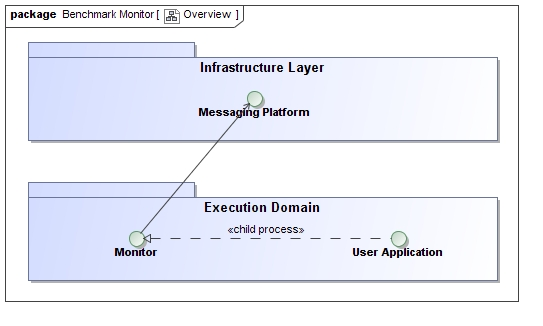
\includegraphics[scale=0.4]{../Diagrams and Charts/Overview/BenchmarkInfrastructure.jpg}
  \caption{A high-level overview of the software architecture for the Benchmark Service}
  \label{fig:benchmarkInfrastructure}
  \end{center}
\end{figure}


\subsubsection{Access and Integration Requirements}
\label{sec:accessIntegrationRequirementsManagementSystem}
\paragraph{Access Channels}
The access channel will only be through a messenging service to the managment service.
\begin{itemize}
	\item Messenging Service to Managment Service
\end{itemize}

\subparagraph{Messenging Service to Managment Service}
The system will expose a further access channel to be used by the so-called
"Management Client". This access channel will be
utilizing a message bus architecture to deliver messages between the benchmark
service and the management backend system.

This access channel will however not be accessable to end users.

\paragraph{Integration Channels}
The various integration channels of the benchmarking system
\begin{itemize}
	\item Integration with a persistence provider
	\item Integration with the human access channels, such as web and
		mobile interfaces
	\item Integration with the message bus architecture
	\item Integration with Linux Containers
\end{itemize}

The integration with the persistence provider is required as we need to persist
the measurements obtained with the benchmarking service.\\\\

The final intergration required by the benchmarking system is that of integration
with the message bus.

Once a program is uploaded via the a managment service, it will be deployed
to the benchmarking cluster in a Linux Container (LXC), upon which the
benchmarking will commence.  The reason for utilizing Linux containers is in
order to meet the security quality requirements as provided in
section \ref{sec:securityQualityRequirement}.

\subsubsection{Quality Requirements}
\label{sec:qualityRequirementManagementSystem}
The quality requirement are the requirements around the quality attributes of
the systems and the services it provides. This includes requirements like
maintainability, flexibility, extensibility, performance, scalability, security,
auditability, usability and testability requirements.
\paragraph{Security}
Security within the benchmarking service should concern the fact that user programs
are not allowed to manipulate the underlying system that it is running on.
Therefore we are utilizing Linux Containers.

\paragraph{Flexibility}
\paragraph{Maintainability}
Amongst the most important quality requirements for the system is
maintainability. It should be easy to maintain the system in the future. To this end

\begin{itemize}
\item future developers should be able to easily understand the system,
\item the technologies chosen for the system an be reasonably expected to be available for a long
time,
\item and developers should be able to easily and relatively quickly
	\begin{itemize}
		\item change aspects of the functionality the system provides, and
		\item add new functionality to the system.
	\end{itemize}
\end{itemize}

\paragraph{Scalability}
The system needs to be able to process multiple requests for benchmarking a program,
but not to hinder the results by running simultaneously. Therefore we need to
implement a scheduling algorithm which maximises throughput, without skewing results.

\paragraph{Testability}
All services offered by the system must be testable through
\begin{enumerate}
	\item automated unit tests testing components in isolation using mock objects, and
	\item automated integration tests where components are integrated within the actual environment.
\end{enumerate}

In either case, these functional tests should verify that
\begin{itemize}
	\item the service is provided if all pre-conditions are met (i.e. that no exception is raised)
	\item the correct execption is throw when the corresponding pre-condition
	is violated.
	\item that all post-conditions hold true once the service has been provided.
\end{itemize}

In addition to functional testing, the quality requirements should also be tested.

\paragraph{Integrability}
The system should be able to easily address future integration requirements
by providing access to its services using widely adopted public standards.

\paragraph{Deployability}
\label{sec:systemDeployability}

\section{Container}

\subsection{Architecture Requirements}


\subsubsection{Quality Requirements}
\paragraph{Flexibility}


\paragraph{Maintainability}


\paragraph{Scalability}


\paragraph{Performance}


\paragraph{Reliability}


\subsubsection{Architectural Responsibilities}


\subsubsection{Architecture Constraints}


\subsection{Architecture Design}
\subsubsection{Tactics}

\subsubsection{Architectural Components}

\subsubsection{Frameworks and Technologies}

\paragraph{Concepts and Constraints for Application Components}


\section{Monitor}

\subsection{Architecture Requirements}


\subsubsection{Quality Requirements}
\paragraph{Flexibility}


\paragraph{Maintainability}


\paragraph{Scalability}


\paragraph{Performance}


\paragraph{Reliability}


\subsubsection{Architectural Responsibilities}


\subsubsection{Architecture Constraints}


\subsection{Architecture Design}
\subsubsection{Tactics}

\subsubsection{Architectural Components}

\subsubsection{Frameworks and Technologies}

\paragraph{Concepts and Constraints for Application Components}

